\bookchapter{Глава 49: Настраиваем окружение — Android Studio и первый проект}

\chapterintro{Чтобы дело спорилось, сначала наточи инструмент. В этой главе мы обустроим «кухню»: установим Android Studio, запустим эмулятор, создадим первый в жизни Android-проект и разберём структуру проекта по косточкам. Когда окружение готово, вы впервые увидите, как написанный вами код превращается в кнопку, на которую можно нажать, — этот момент многие запоминают на всю жизнь.}

\booksection{Устанавливаем Android Studio}

Android Studio — официальная интегрированная среда разработки (IDE) от Google, бесплатная и «всё в одном»: написание кода, предпросмотр интерфейса, отладка и сборка — всё здесь. Установка в четыре шага:

\begin{enumerate}
  \item Откройте официальный сайт developer.android.com/studio и скачайте последнюю стабильную версию (на август 2026 года — выпуск после Narwhal; есть для Windows/Mac/Linux);
  \item Запустите установщик и идите «Далее» — мастер установки автоматически включит Android SDK и компоненты эмулятора;
  \item При первом запуске скачайте компоненты SDK по подсказкам (галочки по умолчанию сойдут; понадобится несколько минут и несколько гигабайт диска);
  \item Когда всё завершится, вы увидите экран приветствия — поздравляем, «кухня» готова.
\end{enumerate}

\begin{tcbwarn}{Внимание: держите в уме требования к железу}
Android Studio — обжора оперативной памяти: желательно от 16 ГБ ОЗУ (пойдёт и 8 ГБ, но эмулятор будет подтормаживать), не меньше 20 ГБ на диске, процессор с поддержкой виртуализации (в BIOS включить VT-x/AMD-V). Если компьютер совсем старый, вместо эмулятора можно использовать «отладку на реальном устройстве» (об этом в четвёртом разделе главы) — так даже плавнее.

\end{tcbwarn}

\booksection{Создаём первый проект}

На экране приветствия нажмите New Project, выберите шаблон Empty Activity (самый чистый шаблон для новичков) и заполните три поля:

\begin{center}
\begin{tabularx}{\linewidth}{|X|X|X|}
\hline
\textbf{Параметр} & \textbf{Что ввести} & \textbf{Пояснение} \tabularnewline
\hline
Name & My First App & Имя приложения — показывается на рабочем столе телефона \tabularnewline
Package name & com.example.myfirstapp & Глобально уникальный идентификатор; по традиции — «домен наоборот», пока оставьте по умолчанию \tabularnewline
Minimum SDK & API 26(Android 8.0) & Минимально поддерживаемая версия, покрывает 95\%+ устройств \tabularnewline
\hline
\end{tabularx}
\end{center}

\begin{center}\small\color{gray}Три вещи, которые заполняются при создании проекта\end{center}

После нажатия Finish Android Studio через Gradle автоматически скачает зависимости и соберёт проект (в первый раз придётся подождать несколько минут, потом будет заметно быстрее). Когда сборка завершится, у вас будет запускаемое приложение — правда, пока оно умеет лишь показывать строку «Hello Android!».

\begin{tcbinfo}{Совет: тонкости имени пакета}
Имя пакета (package name) — как «номер паспорта» приложения: уникально в мире, а после публикации уже не меняется. Для личных упражнений сойдёт com.example.xxx; для настоящего продукта — ваш собственный «домен наоборот» (например, com.вашеимя.имяприложения). Публиковать под com.example нельзя — магазин отклонит.

\end{tcbinfo}

\booksection{Запускаем: эмулятор и реальное устройство}

Код написан — теперь нужен «телефон», на котором он запустится. У вас два варианта:

\booksubsection{Эмулятор (Emulator)}

Эмулятор виртуально создаёт Android-телефон внутри компьютера. В Android Studio откройте Device Manager Create Device, выберите устройство (рекомендуется серия Pixel) выберите образ системы (с Google APIs) скачайте запустите. Затем нажмите зелёный треугольник Run на панели инструментов — через несколько секунд на экране «телефона» появится ваше приложение.

\booksubsection{Отладка на реальном устройстве (более рекомендуемая)}

Реальный телефон — всегда самая подлинная тестовая среда: плавность скролла, настоящая сеть, настоящие датчики — эмулятор этого не передаст. Отладка на реальном Android-устройстве несложна:

\begin{enumerate}
  \item На телефоне откройте [Настройки] [О телефоне] и семь раз подряд нажмите «Номер сборки» — включатся «Параметры разработчика»;
  \item В [Параметрах разработчика] включите «Отладка по USB»;
  \item Соедините телефон с компьютером кабелем и во всплывающем окне на телефоне выберите «Разрешить отладку по USB»;
  \item Вернитесь в Android Studio: ваш телефон появится в выпадающем списке устройств на панели инструментов — нажмите Run.
\end{enumerate}

\textbf{Осторожно: не держите отладку по USB включённой постоянно}\par

Отладка по USB — это как «чёрный ход» в телефон для компьютера. Заряжаясь в общественных местах или подключаясь к чужому компьютеру, обязательно выключайте отладку по USB, чтобы никто не смог прочитать ваши данные. Приучите себя: попользовались — выключили.

\booksection{Разбор структуры проекта: за что отвечает каждый файл}

При первом открытии проекта дерево файлов слева может вскружить голову. Спокойно: в повседневной разработке 90\% времени вы соприкасаетесь только с этим:

\begin{center}
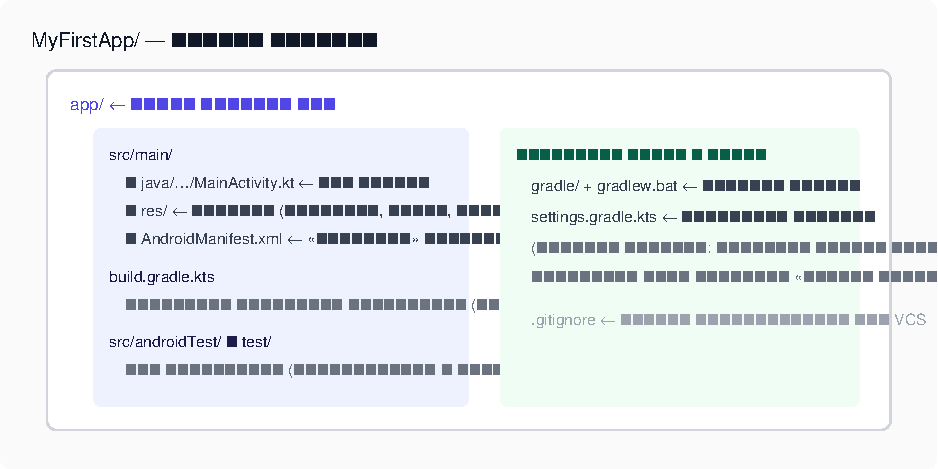
\includegraphics[width=0.92\linewidth]{figures/fig-di-si-shi-jiu-zhang-1}
\\[2pt]\small Рисунок 2: структура проекта, которую обязан понять новичок (запоминалка: трогаем только каталог app/)
\end{center}

\begin{itemize}
  \item MainActivity.kt: «входная дверь» приложения. Пользователь нажимает на иконку — первым просыпается именно этот класс. В текущем шаблоне он отвечает за показ «Hello Android!».
  \item AndroidManifest.xml: «домовая книга» приложения — объявляет, как оно называется, какая у него иконка, какие есть экраны и какие нужны разрешения (камера, местоположение и т. д.).
  \item Каталог res/: склад ресурсов — здесь хранятся картинки, иконки, строки, цвета. Хранить текст в файлах ресурсов, а не зашивать его в код — хорошая практика Android (легко менять язык и тему).
  \item build.gradle.kts: «рецепт сборки» — объявляет минимально поддерживаемую версию и библиотеки-зависимости (например, Compose).
\end{itemize}

\booksection{Проба пера: меняем «Hello» на своё имя}

Откройте MainActivity.kt — увидите код, сгенерированный из шаблона Compose. Найдите строку Text(“Hello Android!”) и замените текст в кавычках на своё имя, например Text(“Привет, Аня! Это моё первое приложение”), а затем нажмите Ctrl+R (на Mac — Cmd+R), чтобы запустить заново. Через несколько секунд на эмуляторе появится ваше имя.

\begin{lstlisting}[language=Kotlin]
setContent {
    MyFirstAppTheme {
        Surface(modifier = Modifier.fillMaxSize()) {
            // v замените это на свой текст
            Text("Привет, Иван! Это моё первое приложение")
        }
    }
}
\end{lstlisting}

Поздравляем: вы только что прошли полный цикл «изменил код собрал установил запустил». Этот цикл и есть ваши будни разработчика на все дни вперёд. Куй железо, пока горячо: попробуйте ещё что-нибудь поменять — увеличить шрифт, поменять цвет. В следующей главе мы узнаем, откуда берутся эти «магии».

\booksection{Скорая помощь при типичных ошибках: «приёмный покой» новичка в первые две недели}

На этапе настройки окружения и первой сборки вы почти наверняка встретите три следующие ошибки. Не паникуйте — против каждой есть лекарство:

\begin{center}
\begin{tabularx}{\linewidth}{|X|X|X|}
\hline
\textbf{Симптом ошибки} & \textbf{Частая причина} & \textbf{Лекарство} \tabularnewline
\hline
Gradle sync failed / зависимости качаются медленно & Проблемный доступ к репозиториям по сети & Настройте для Gradle зеркала репозиториев (maven-зеркала Aliyun/Tencent Cloud): найдите в интернете готовую инструкцию по зеркалам Gradle для Китая и следуйте ей \tabularnewline
Отсутствуют компоненты SDK & При установке была пропущена загрузка SDK & Settings SDK Manager: доустановите недостающие платформы и инструменты \tabularnewline
Эмулятор не запускается / чёрный экран & Не включена виртуализация, повреждён образ & Включите в BIOS VT-x/AMD-V; удалите эмулятор и создайте заново; либо сразу отлаживайтесь на реальном устройстве \tabularnewline
\hline
\end{tabularx}
\end{center}

\begin{center}\small\color{gray}Таблица скорой помощи при ошибках окружения у новичков\end{center}

\begin{tcbinfo}{Совет: методология поиска ошибок}
Первая строка сообщения об ошибке — самая ценная: скопируйте её в поисковик как есть, добавив ключевые слова «android studio». Не ищите расплывчатое «не могу настроить окружение», а ищите конкретную ошибку вроде «Gradle sync failed: Could not resolve com.android.tools.build». Точный вопрос — точный ответ.

\end{tcbinfo}

\begin{tcbpractice}{Попробуйте сами: пройдите свой список «ритуалов разработчика»}
1) Установите Android Studio и запустите эмулятор; 2) запустите своё приложение на реальном телефоне и сделайте памятный скриншот; 3) замените текст Hello на своё имя; 4) заархивируйте проект на хранение. Сделав эти четыре шага, вы можете объявить друзьям: я тоже Android-разработчик (скриншот прилагается).

\end{tcbpractice}

\begin{tcbsummary}{Краткие итоги главы}
\begin{itemize}
  \item Android Studio = официальная бесплатная IDE; советуем 16 ГБ ОЗУ + 20 ГБ диска + включённая виртуализация
  \item Три основы нового проекта: имя, имя пакета (уникально в мире; com.example не публиковать), минимальный SDK (от API 26)
  \item Два способа запуска: эмулятор (виртуальный телефон в компьютере) и реальное устройство (включить отладку по USB, после работы выключить)
  \item Запоминалка по структуре: трогаем только каталог app/ — MainActivity.kt входная дверь, Manifest — домовая книга, res/ — склад ресурсов
  \item Будни разработки = изменить код Run посмотреть результат — и так по кругу
\end{itemize}

\end{tcbsummary}
